% \documentclass[a4paper,11pt]{report}
% \usepackage[T1]{fontenc}
% \usepackage[utf8]{inputenc}
% \usepackage{lmodern}
% \usepackage[francais]{babel}
% \usepackage{graphicx}
% \usepackage{array}

\documentclass[a4paper, titlepage]{livret}

\usepackage[utf8]{inputenc} % accents
\usepackage[T1]{fontenc}      % caractères français
\usepackage{geometry}         % marges
\usepackage[francais]{babel}  % langue
\usepackage{graphicx}         % images
\usepackage{verbatim}         % texte préformaté
\usepackage{array}
\usepackage{graphicx}


\setlength{\parindent}{0cm}
\setlength{\parskip}{1ex plus 0.5ex minus 0.2ex}
\newcommand{\hsp}{\hspace{20pt}}
\newcommand{\HRule}{\rule{\linewidth}{0.5mm}}

\title{Data wars }

\author{Guillaume LAROYENNE, Nathan PRETOT \\ Jeremy RENAUD, Tom SALVI, Pierre VALENZA}

%
%
% \title{Rapport de stage}      % renseigne le titre
% \author{Prénom Nom}           %   "   "   l'auteur
% \date{18 juin 2007}           %   "   "   la future date de parution
%
%          % affiche un rappel discret (en haut à gauche)
%                               % de la partie dans laquel on se situe
%


\begin{document}
\begin{titlepage}
  \begin{sffamily}
  \begin{center}

    % Upper part of the page. The '~' is needed because \\
    % only works if a paragraph has started.
  %  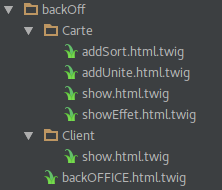
\includegraphics[scale=0.04]{Assets/backOff.png}~\\[1.5cm]

    \textsc{\LARGE IUT informatique de Belfort-Montbéliard}\\[2cm]

    \textsc{\Large Rapport de projet tuteuré}\\[1.5cm]

    % Title
    \HRule \\[0.4cm]
    { \huge \bfseries Data wars\\[0.4cm] }

    \HRule \\[2cm]
    
\includegraphics[scale=0.4]{../mainPageimg.png}
    \\[2cm]

    % Author and supervisor
    \begin{minipage}{0.4\textwidth}
      \begin{flushleft} \large
        Guillaume \textsc{LAROYENNE}, \\ Nathan \textsc{PRETOT}, \\ Jeremy \textsc{RENAUD}, \\ Tom \textsc{SALVI}, \\ Pierre \textsc{VALENZA}
      \end{flushleft}
    \end{minipage}
    \begin{minipage}{0.4\textwidth}
      \begin{flushright} \large
        \emph{Tutrice :} Mme. \textsc{Deschinkel} \\
      \end{flushright}
    \end{minipage}

    \vfill

    % Bottom of the page
    {\large 1\ier{} Octobre 2016 — 27 Mars 2016}

  \end{center}
  \end{sffamily}
\end{titlepage}





\maketitle
\tableofcontents

\chapter{Remerciement}
Nous tenons à remercier notre enseignante tutrice, Madame Karine Deschinkel qui nous a été d'une aide précieuse et qui nous a consacré du temps, notamment pour définir des règles précises.

Nous remercions également Madame Corinne PATERLINI, pour ses cours sur la dynamique de groupe et ceux sur la gestion de conflits.

\chapter{Introduction}

	Le projet de deuxième année de DUT informatique est important. Le choix du sujet ainsi que l’équipe de projet le sont aussi. Outre le fait que le projet constitue une note importante pour notre moyenne du semestre, ce dernier peut être un plus pour notre avenir professionnel, ou même pour notre stage. Le choix du sujet, même si il a été plutôt rapide à trouver, a été très long à définir entièrement, en effet fixer les grandes lignes du sujet a été aisé : nous voulions un jeu de plateau, se jouant avec des cartes, et jouable en réseau. Cependant, pour délimiter entièrement le sujet il nous a fallut un temps conséquent qui s'explique par la création d'une multitude de règles pour rendre le jeu intéressant et attractif. De notre point de vue, ce projet avait donc un potentiel très intéressant car nous pouvions appliquer nos connaissances dans de nombreux domaines : en effet il mêle du réseau, de la base de donnée ainsi que du java. Mais également du PHP puisque nous avons dû réaliser un site web.
	
	L'équipe de projet est constituée de Guillaume LAROYENNE, de Nathan PRETOT, de Jérémy RENAUD, de Tom SALVI et de Pierre VALENZA.
	
	Ce projet a été encadré par Karine DESCHINKEL, enseignante à l'IUT de Belfort-Montbéliard. 

\chapter{Cahier des charges}
  Pour réaliser le cahier des charges, nous avions deux principaux types de contraintes, les contraintes liées a la programmation, ainsi que les contraintes fonctionnelles.
  \section{Les contraintes de programmation}
    \begin{description}
      \item[Intégrer une base de données :] Une base de données doit stocker les informations des différentes cartes.
      \item[Le site web :] Le joueur peut décider des cartes qu’il va utiliser lors de sa prochaine partie depuis un site web, relié a la base de données mais non directement relié a l’application.
    \end{description}
    
      \section{Les contraintes fonctionnelle :}
      \begin{description}
        \item[Le plateau :] 	La taille du plateau varie selon le nombre de joueurs
	Tous les éléments se trouvant sur le plateau ne font qu’une seule case.
	Une case ne peut contenir qu’un seul élément.
	Le plateau contient des obstacles, des quartiers généraux et des bâtiments de ressources 			avant que la partie ne commence. 
        \item[Les unités : ]	Une unité ne doit prendre qu’une seule case.
	Une unité peut être posée uniquement sur une case adjacente a un bâtiment contrôlé.
	Une unité dispose d’un coût, de points d’attaque, de points de vie, de points de mouvement, 		d’une portée, d’une image, et d’un nom.
	Une unité peut disposer d’un effet.
	Une unité est détruite lorsque ses points de vie atteignent zéro.
	Une unité peut se déplacer et attaquer.
        \item[Les sorts :] Un sort dispose d’un coût et d’un effet.

        \item[Les bâtiments de ressources :]Un bâtiment de ressource peut être soit neutre soit contrôlé par un joueur, lorsqu’une unité 		se trouve sur une case adjacente a lui
        \item[Les joueurs :] 	Chaque joueur dispose d’un ensemble de cartes appelé deck qu’il a lui même construit 		depuis le site internet.
	Chaque joueur dispose de ressources, obtenues en contrôlant des bâtiments.
	Chaque joueur commence avec un quartier général.
	Lorsque le quartier général d’un joueur est détruit, ses unités sont détruites, et il perd la 			partie
        \item[Les obstacles :] Un obstacle ne peux pas être détruit.
        \item[Les ressources :] Chaque joueur dispose d’une réserve de ressources. 	Chaque joueur reçoit des ressources en fonction du nombre de bâtiment qu’il contrôle au début de son tour. 
        \item[Les conditions de victoire : ] La partie se termine lorsqu’il ne reste plus qu’un joueur en vie.
        \item[Les cartes : ] Lorsqu’une carte est utilisée, son coût est déduit de la réserve de ressources du joueur qui l’a 		posé, puis la carte retourne à la fin du deck.
        \item[Le deck : ]	Un deck constitue un ensemble de carte.
	Un deck est propre a chaque joueur.
	Le deck est constitué depuis le site internet avant la partie.
	      \item[Le quartier général : ]Chaque joueur commence avec un quartier général. Il fournit des ressources.
	Un quartier général de peut pas changer de propriétaire .
        
      \end{description}
    
    
    
    
    

\chapter{Mise en œuvre}
  \section{Logiciels et méthodes utilisés}
  \subsection{Organisation du projet}
     \begin{description}
       \item[Logiciel de gestion de versions :] nous avons utilisé \textit{git} et la plateforme \textit{GitHub} pour gérer le partage des fichiers et la gestion des versions. Nous avons utilisé ceci car, l'ayant appris en cours, tout les membres du projet étaient capable de l'utiliser.
       \item[Communication :] pour la communication d'information importante et d'information durable, l'utilisation de mail ou encore de système de discussion instantanée tel que \textit{messenger}. En plus de tout ceci, l'utilisation du logiciel de discussion \textit{Discord} nous a permit de parler du projet de vive voix.
       \item[Répartition des tâches :] pour la répartition des tâches et l'organisation du projet, nous nous sommes servis du site \textit{Trello}. Son interface simple, mais efficace, nous a permit de suivre l'avancé du projet.
     \end{description}
  
  \subsection{Jeu}
    \begin{description}
      \item[Langage de programmation :] \textit{Java} fut choisit pour plusieurs raisons, notamment, étant le langage le plus utilisés lors de notre formation, tout les membres de notre groupe avait un niveau équivalent sur celui-ci. De plus, la création d'une interface graphique en \textit{Java}, ayant été vue en cours, était donc connu par notre groupe.   
      \item[Base de données :] nous avons décidé d'utiliser \textit{MySQL}. Nous avons fait ce choix pour la simplicité d’intégration avec \textit{java} via la bibliothèque \textit{mysql-connector}.
      
    \end{description}
  
    \subsection{Interface}
    \subsubsection{Le Paradigme MVC}
    Nous avons structuré notre projet avec le paradigme MVC ( Modèle, Vue, Contrôleur), car ce format s'adapte parfaitement au jeu en tour par tour. En effets il permet de juste envoyer la partie modèle avec le réseau sans toucher ni aux contrôleurs ni à la vue.   
    \subsubsection{La bibliothèque graphique Java Swing}
    Nous avons décidé d'utiliser la bibliothèque graphique Java Swing car nous l'avions déjà utiliser sur plusieurs projets et que c'est la technologie que nous maitrisions le plus.
    \subsubsection{Logiciels}
    Voici les différents logiciels utilisés pour réaliser les graphismes.

    \begin{description}
      \item[Gimp :] Nous avons utilisé ce logiciel pour la modification des images de la vue. Nous avons choisi ce logiciel car c'est un logiciel gratuit et que l'on maitrisait déjà un peu. 
      \item[Inkscape :] Nous avons utilisé ce logiciel pour la création des images de la vue. Nous avons choisi inkscape car c'est un logiciel libre qui permet de faire du dessin vectoriel, et donc de pouvoir facilement redimensionner les images. 
    \end{description}



\subsection{Réseau}

\subsubsection{Langage utilisé}
Le langage Java est utilisé pour le serveur et le client pour sa simplicité. En effet java permet un échange des données extrêmement simple grâce à la sérialisation de ses objets. De plus la création des connexions réseau se fait rapidement.
En utilisant ce langage, la communication entre les programmes a donc pu être réalisée rapidement, permettant aux développeurs de se consacrer davantage sur les protocoles.

\subsubsection{Bibliothèques utilisée}
Les bibliothèques utilisées pour le serveur sont :
\begin{enumerate}
  \item GraphStream, pour la visualisation de l'état du serveur sous forme de graphe. Car cette librairie est très similaire à la librairie PHP que nous avons utilisée aux parts avant.
  \item MySQL Connectors, pour la communication avec la base de donné. Car cette librairie contient de nombreux outils compatibles avec Java Swing.
  \item Java Zoom, pour la lecture de fichiers audio. Car cette librairie est très simple d’utilisation et contient une bonne documentation.
\end{enumerate}

\subsubsection{Test unitaire}
Pour pouvoir identifier rapidement les erreurs éventuelles dans les protocoles, ainsi que des failles de sécurité, des tests unitaires ont été réalisés. Ces tests ont été réalisées avec la librairie JUNIT. 


	

  \section{Répartition du travail}
    Ce projet mettant en œuvre une grande diversité de domaine (site web, jeu, serveur, base de données, graphisme), nous n'avons donc pas eu d'autres choix que de répartir notre effectif sur les différents domaines. Laissant ainsi presque tout les domaines (à part modèle) couvert par une seule personne, nous laissant la disposition suivante :
    \begin{description}
      \item[Jeremy : ] implémentation des interfaces et des contrôleurs.
      \item[Tom : ] travail sur une partie du modèle du jeu.
      \item[Guillaume :] modélisation et création du serveur et des communications réseaux.
      \item[Pierre :] création du site web.
      \item[Nathan :] modélisation et création de la base de données. Modélisation du jeu et réalisation d'une partie de celui-ci.
    \end{description}
    
    \begin{figure}[th]
      \begin{center}
        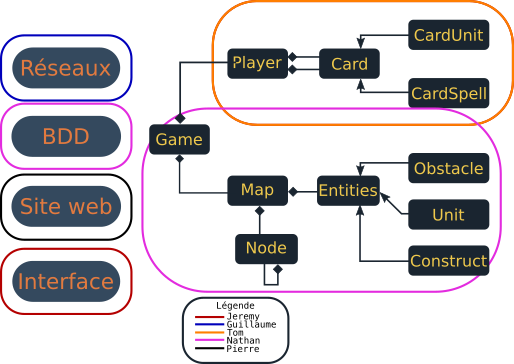
\includegraphics[scale=0.365]{Assets/UMLRepartition.png}
        \caption{Répartition du travail}
        \label{RepTravail}
      \end{center}
    \end{figure}
    
    De plus des éléments du domaine informatiques, notre projet nous a demandé la création entière d'un jeu, nous demandant une réflexion autours des règles et fonctionnalités de celui-ci, ainsi que de créer des cartes innovantes pour celui-ci. Cette partie à été endossée par l'ensemble de l'équipe.
    
    	\subsection{Site internet}

 	\textbf{Langage de programmation :} PHP est un langage simple de programmation qui est le plus utilisé pour le développement de sites web. Nous l'avons aussi utilisé afin d'exploiter une base de données.

	\textbf{Framework :} nous avons choisi d'exploiter un micro-framework : Silex. Du fait qu'il soit minimaliste il laisse beaucoup de liberté aux développeurs comme le fait de ne pas imposer une architecture. De plus il offre un ensemble de services destiner aux contrôles de données.

	\textbf{Framework CSS :} Bootstrap est un kit CSS créer par les développeurs de Twitter. Il permet de développer un site reponsive, donc pouvant s'adapter sur différents appareils, facilement et efficacement.

    
  \section{Gestion du temps}
    Le projet a débuté sur la conception du jeu. C'est-à-dire la création des règles, ainsi que les éléments de modélisation au niveau informatique ( MCD, UML, etc...).  C'est étape, qui a durée un mois et demis, fut suivit du début de la phase de programmation du réseau et du jeu. La partie interface commença un peu plus tard, car elle nécessitais d'avoir une partie du modèle de terminée pour commencer. Le site web ne commença qu'a partir de janvier car celui-ci n'était pas prévus dans le travail initiale. Une première version du jeu en mono-poste fut terminée au milieu des vacances de février, suivis de près par la version réseau.
    \begin{figure}[th]
      \begin{center}
        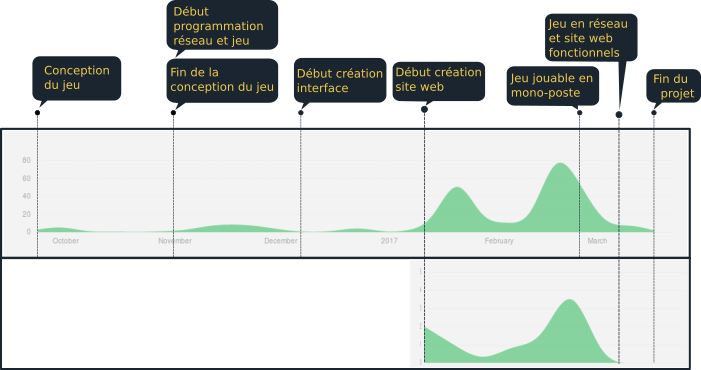
\includegraphics[scale=0.5]{Assets/gestionTemps.png}
        \caption{Gestion du temps par rapport à la courbe des \textit{commits} \textit{GitHub}}
        \label{RepTime}
      \end{center}
    \end{figure}
  


\section{Rendu}
\subsection{Les composants du projet}



	\subsection{Un site internet}

	\paragraph{}
        Data wars est un jeu qui utilise une base de données contenant les informations des utilisateurs ainsi que les cartes qui leur sont nécessaires. Pour accéder à ces données et les modifier, nous avons mis en place un site web réalisé en PHP afin d'y apporter un niveau de sécurité suffisant lors de sa modification. L'architecture du site est réalisé en Modèle-Vue-Contrôleur (MVC) ce qui améliore la facilité de maintenance du site, d’ailleurs pour la vue nous avons fait le choix d'en faire un site \textit{responsif} afin d'y accéder depuis n'importe quel appareil. 

	\subsubsection{Partie administrateur} 
	\paragraph{}

    	\begin{figure}[th]
      	 \begin{center}
          
\includegraphics[scale=0.25]{Assets/navbar_admin.png}
          \caption{Barre de navigation côté administrateur}
          \label{RepTravail}
         \end{center}
        \end{figure}

	 La première du site n'est accessible que par les administrateurs afin de pouvoir mettre à jour : 
	\begin{enumerate}
		\item les cartes
		\item les joueurs
		\item les effets
	\end{enumerate}Il a donc été nécessaire d'y installer une sécurité afin que les données enregistrées soient correctes pour ainsi éviter que des conflits apparaissent. Pour cela nous utilisons un framework : Silex, qui offre donc des services pour mettre en place des contraintes qui doivent être respectées par l'utilisateur pour que les données saisies soient envoyées dans la base de données.



	\subsubsection{Partie joueur}
	\paragraph{}

	\begin{figure}[th]
      	 \begin{center}
          
\includegraphics[scale=0.25]{Assets/navbar_joueur.png}
          \caption{Barre de navigation côté joueur}
          \label{RepTravail}
         \end{center}
        \end{figure}

      La seconde partie du site est donc accessible par les joueurs qui d'ailleurs devront créer leur compte sur le site. À partir d'ici il est nécessaire de respecter les contraintes du jeu : 

	\begin{enumerate}
		\item la taille du deck a une limite à ne pas dépasser
		\item une carte n'est pas dans le deck ou l'est maximum une fois
	\end{enumerate}Pour cela on empêche tout simplement l'ajout lorsque cette limite est atteinte à l'aide de requêtes SQL qui compte et compare les cartes du jeu avec celles présentes dans le deck.
	
	\paragraph{}
	L'objectif principal a donc été de réaliser une vue qui soit agréable pour la construction des decks. Ainsi la modification se fait sur une seule page où le deck du joueur, les cartes du jeu, et une vue détaillée de la carte sélectionnée sont visibles. De cette manière le joueur peut donc naviguer entre les cartes de manière aisée. Toutefois lorsqu'une action est effectuée la page doit se recharger, on pourrait donc améliorer cette partie pour rendre la navigation plus fluide aux joueurs en y ajoutant du \textit{Javascript}.



	\subsection{Un système réseau indépendant du modèle :}
	
	Ce système réseaux, est à l'heure actuelle capable de s'adapter à n'importe quel modèle de jeux en tour par tour, le rendant ainsi totalement autonome. Il permet la création d'un groupe, qui a une capacité de 4 personnes, par une joueur nommé l’hôte. Celui-ci peut inviter jusqu'à trois autres joueurs via une interface (Figure~\ref{interface reseau}), qui recevront une invitation qu'ils devront accepter. Ces invitations, limitées dans le temps, évite l'attente éventuelle d'un joueur. Une fois que les joueurs sont tous dans le groupe, appelé \textit{<<lobby>>}, l'hôte peut lancer la partie. Le programme va alors lancer le jeu et laisser place à celui-ci. Le réseau ne sera désormais appelé seulement lors de la fin de tour des joueurs, où il se chargera de transmettre le modèle au autre joueurs.
	
	 \begin{figure}[th]
	\begin{center}
	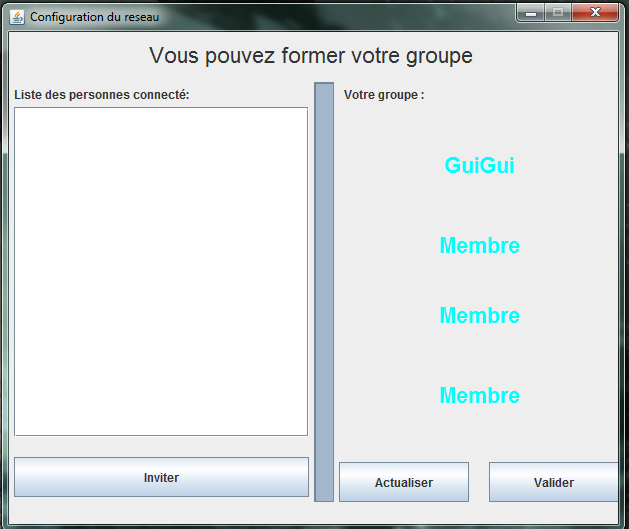
\includegraphics[scale=0.4]{Assets/connection3.png} 
	\caption{Interface du module réseau}
     \label{interface reseau}
      \end{center}
    \end{figure}

	\newpage
	
	\subsection{Un jeu jouable en Réseau de 2 à 4 joueurs.}
	
	Lorsque la partie commence, chaque joueur se voit attribuer les cartes correspondantes à son choix sur le site web. Cinq lui sont distribuées dans leurs mains (Figure~\ref{cartesJoueur}) tandis que les autres sont misent de coté pour devenir la pioche, ou encore appelé le <<deck>>. 
	 \begin{figure}[th]	
	\begin{center}
	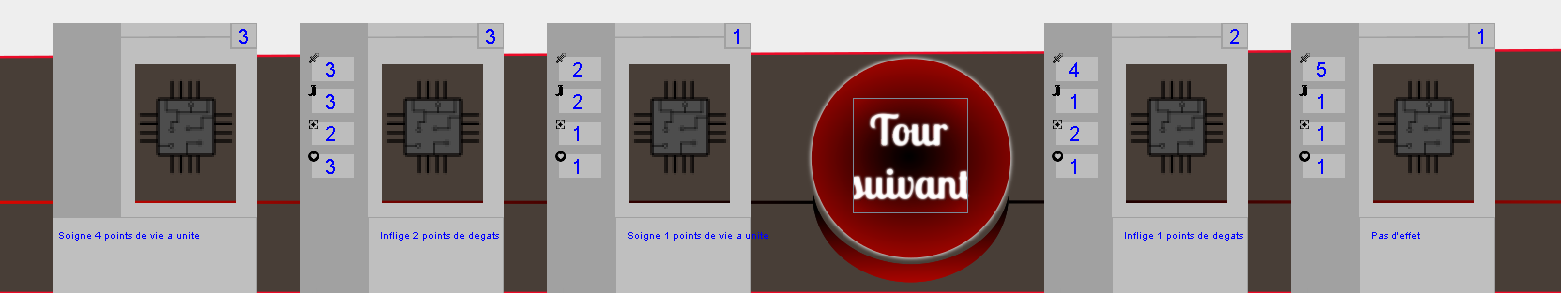
\includegraphics[scale=0.4]{Assets/mainJoueur.png} 
	\caption{main du joueur}
     \label{cartesJoueur}
      \end{center}
    \end{figure}


	
	 Le joueurs commençant peut dès à présent jouer ces cartes selon sa quantité de ressource.une fois celle-ci joué, il peut voir apparaître l'unité ou l'effet du sort de la carte sélectionnée. Une fois son tour terminé, il peut le passer en appuyant sur le bouton <<fin de tour>>. C'est alors au tour des autres joueurs de jouer. Une fois un tour table complet effectué, le joueur pour déplacement l'unité qu'il avait créé le tour précèdent (Figure~\ref{MouvementUnité}). Cette unité pourra lui servir à en attaquer d'autres, ou encore à capturer des bâtiments de ressources (Figure~\ref{CaptureBatiment}) qui lui permettra de gagner plus de ressource.
	 	
	 
	  \begin{figure}[th]
	 \begin{center}
	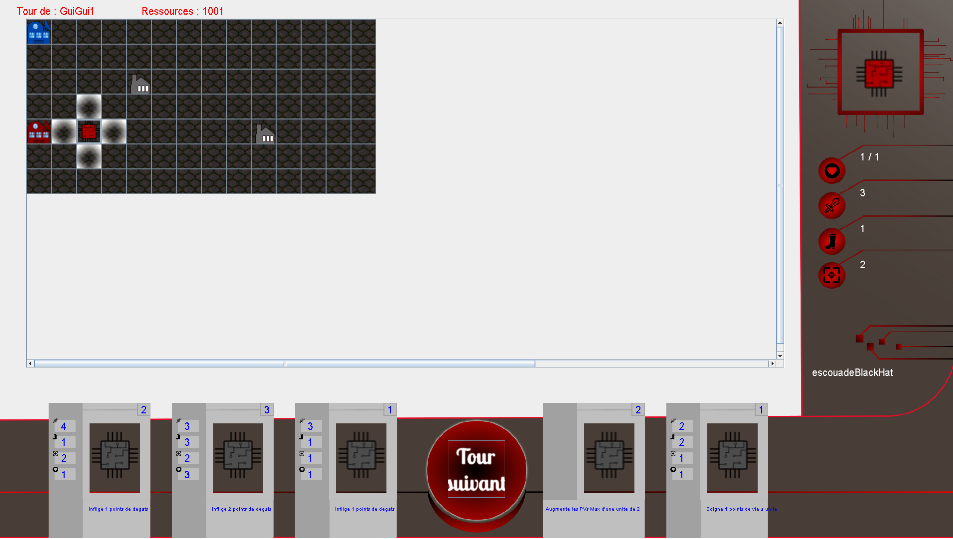
\includegraphics[scale=1]{Assets/UniteeSelectMove.png} 
	\caption{déplacement d'une unité}
     \label{MouvementUnité}
      \end{center}
    \end{figure}

	 

	

	
	 \begin{figure}[th]
	\begin{center}
	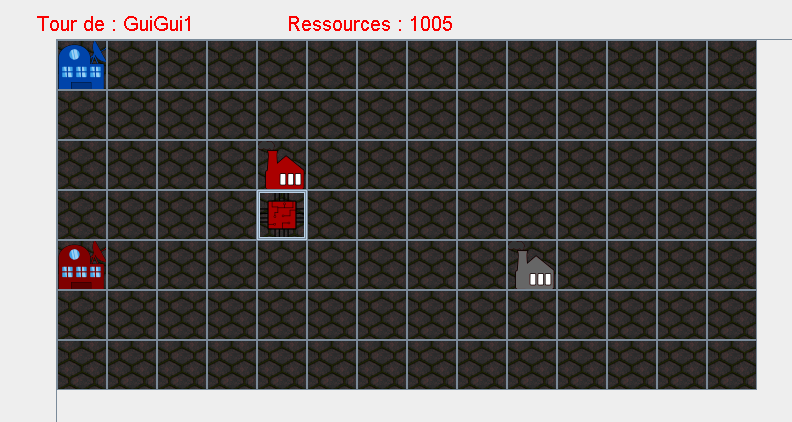
\includegraphics[scale=0.5]{Assets/CaptureSucces.png} 
	\caption{Capture d'un bâtiment}
     \label{CaptureBatiment}
      \end{center}
    \end{figure}
	
	 Plusieurs tours ce sont écoulés, notre joueur est sur le point de détruire le derniers QG adverse. Il va par conséquent gagner la partie. L'écran de jeu va se fermer et les joueurs seront redirigée vers la fenêtre de connexion du réseaux.
	

  
  \chapter{Bilan}
    \section{Bilan pédagogique}
      Ce projet nous a permit de renforcer nos acquis dans des langages tels que \textit{Java}, \textit{MySQL} ou encore \textit{PHP} avec le \textit{framework} <<silex>>. Mais ce projet nous également permit d'acquérir de nouvelle connaissance, notamment comment lié \textit{Mysql} a \textit{Java}, ou encore la communication réseaux en \textit{Java}. Ce projet, et quelques mésaventures avec des modifications de code altérant le bon fonctionnement du programme, nous a appris que la pratique du test logiciel était importante pour la programmation d'un jeu.
      
    \section{Bilan technique}
       Nous avons à l'heure actuelle un programme fonctionnel malgré quelques failles notamment dû à un manque de rigueur dans la gestion des contrôleurs, mais également de quelques problèmes avec les effets. Certains de ceux-ci ne s'appliquent pas. Si notre programme reste viable dans le fond, la forme reste encore à améliorer. En effet, toutes les cartes n'ont pas encore d'images et l'interface générale du reste minime. Les points évoqués précédemment correspondent aux potentielles voix d'améliorations du projet.
       
 \chapter{Conclusions}
 	Nous avons rencontrés plusieurs types de difficultés lors de ce projet, principalement duent problèmes d’implémentation des règles. Nous avons réussi a surmonter ces problèmes notamment en réalisant une maquette papier sous les conseils de notre professeur-encadrante ainsi qu’en modifiant certaine règles pour les adapter a une version numérique du jeu.
 	
	Malgré quelques tensions d’ordre humain, nous avons su nous reprendre spécifiquement grâce au cours sur la dynamique de groupe ainsi que ceux sur la gestion des conflits. 
	
	Le projet n’a pas atteint exactement la forme que nous souhaitions lui donner, et ce à cause d’un manque de temps évident qui s’est transformé en une démotivation pour certains membres du groupes. 
	Pour conclure ce projet a été enrichissant pour nos connaissances car ils nous a permis de travailler plusieurs langages. Mais également d’avoir une expérience significative sur la gestion d’un projet et d’un groupe. 

\end{document}
